\documentclass[11pt]{article}
\usepackage{geometry}                % See geometry.pdf to learn the layout options. There are lots.
\usepackage{amsmath}
\usepackage{amsthm}
\geometry{letterpaper}                   % ... or a4paper or a5paper or ... 
%\geometry{landscape}                % Activate for for rotated page geometry
%\usepackage[parfill]{parskip}    % Activate to begin paragraphs with an empty line rather than an indent
\usepackage{graphicx} 
\usepackage{amssymb}
\usepackage{setspace}
\usepackage{hyperref}
\usepackage{dsfont}
\usepackage{float}
\usepackage{epstopdf}
\usepackage{amsmath}
\usepackage{mathtools}
\usepackage{tabu}
\usepackage{color}
\usepackage{import}
\usepackage{pdfpages}
\usepackage{listings}
\DeclareGraphicsRule{.tif}{png}{.png}{`convert #1 `dirname #1`/`basename #1 .tif`.png}

\newtheorem{thm}{Theorem}[section]
\newtheorem{exa}[thm]{Example}
\newtheorem{lem}[thm]{Lemma}
\newtheorem{cor}[thm]{Corollary}
\newtheorem{prop}[thm]{Proposition}
\newtheorem{conj}[thm]{Conjecture}
\newtheorem{prob}[thm]{Problem}

\bibliographystyle{plain}


\usepackage{hyperref}
\hypersetup{
    colorlinks,
    citecolor=black,
    filecolor=black,
    linkcolor=black,
    urlcolor=black
}

%\counterwithin*{equation}{section}
%\counterwithin*{equation}{subsection}



\newcommand{\Z}{\mathbb{Z}}
 
\begin{document}

\setlength{\abovedisplayskip}{0pt}
\setlength{\belowdisplayskip}{5pt}
\setlength{\abovedisplayshortskip}{0pt}
\setlength{\belowdisplayshortskip}{12pt}

\title{{\bf{Cover Times of Random Walks}} 
~ \\
  MATH 0710 Thesis}   

\author{Nick Bermingham}
\date{\today}

\maketitle

\begin{abstract}
If a random walk is performed on a connected graph, a cover time is the number of steps required for each vertex to be visited at least once. To begin, we discuss in simple language a few examples drawn from graph theory, until we find that our developed strategy fails with larger, unstructured graphs. We then look at the cover time distribution of a complete graph with self-edges, and prove that the number of unvisited vertices approaches a Poisson distribution in a special case. Finally, we introduce Pólya's Reccurence Theorem, which states that a simple random walk on a d-dimensional lattice is recurrent for $d = 1, 2$, and transient for $d > 2$. We discuss the 1-dimensional, 2-dimensional, and 3-dimensional components of this theorem using The Cliff Hanger, The Drunk Man, and The Drunk Bird problems, respectively.
\end{abstract}

\newpage

\tableofcontents
\newpage
%
\section{Cover Times}
\subsection{Preliminaries}

\indent \indent We define a graph $G = (V, E)$ with vertex set $V$ and edge set $E$.  We say $\vert V \vert  = n$, and $\vert E \vert  = e$, where \textit{n} and \textit{e} can be infinite. A graph is considered to be \textit{connected} if

\begin{equation}
\forall  v_{1}, v_{2} \in V,\text{ } \exists \{e_{1}, e_{2}, \ldots \} \subseteq E \text{ that connects } v_{1} \to v_{2}.
\end{equation}

Consider the following random walk on graph G. A particle is at a certain \textit{starting-vertex} at time \textit{t}  = 0, which we can denote vertex  \textit{i}. From vertex $i$, the particle can move to any of the vertexes with which this vertex is directly connected at \textit{t}  = 1, each with probability 1/$d_i$, where $d_{i}$ is the number of edges incident to $i$. This process continues for $t = 2, 3, \ldots$ . When each choice in a random walk is made with equal probability, a graph is considered to be \textit{unweighted}. A weighted graph is presented in the discussion of Pólya's Recurrence Theorem, in the Gambler's Ruin problem.

The \textit{cover time} - the expected time until all vertices have been visited - can be expressed as $m_{in}$. We can also call this the \textit{absorption time}.  When determining a simple cover time, we assume that the particle stops when the each vertex has been reached. But what if we wanted to let the walk continue until the particle returns to its starting vertex? We call this the \textit{extended cover time}, and we can express this as \textit{$u_{in}$}. Clearly, \textit{$u_{in} > m_{in}$} for all graphs. 

It can also be of interest to consider the expected time for given number \textit{$k < n$} vertices to be visited. We denote this expected value \textit{$m_{ik}$}, and call it a \textit{partial cover time}. If we wish to again compute the time for the particle to return to the starting vertex, we can denote this \textit{$u_{ik}$} - the \textit{extended partial cover time}. 

All of the different kinds of cover times can be independent of the starting-vertex, and can always be found using an appropriate system of linear equations. This process is explained in the following example, and follow from \cite{BG}.

\subsection{A Special Graph}


\indent \indent To begin, let us examine the graph in figure \ref{fig:specialGraph}, where particle rests at vertex 1 at \textit{t}  = 0. From this starting vertex, the particle can move to vertex 2, 3, or 4 - each with probability 1/3. In order to determine the partial cover time \textit{$m_{13}$}, the expected time until \textit{k} = 3 vertices have been visited, we consider each of the possible first moves for the particle. 

\begin{figure}[H]
\centering
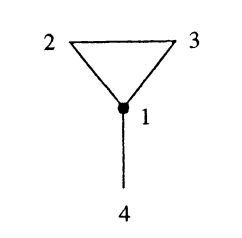
\includegraphics[scale = 0.7]{ASpecialGraph}
\caption{A Special Graph \protect\cite{BG}}
\label{fig:specialGraph}
\end{figure}

\begin{enumerate}
  \item The particle moves first to vertex 2 with probability 1/3. We can denote the expected time required to visit a third and final vertex \textit{a}. This case is represented in the leftmost illustration in figure \ref{fig:specialGraphCases}. The bolded vertex represents the vertex where the particle is present, and the circled vertex represents a vertex that has already been visited.
  \item The particle moves first to vertex 3 with probability 1/3. The expected time to visit a third vertex is again \textit{a}, by symmetry.
  \item The particle moves first to vertex 4 with probability 1/3. We can set the expected remaining time as \textit{b}.
\end{enumerate}

\begin{figure}[h]
\centering
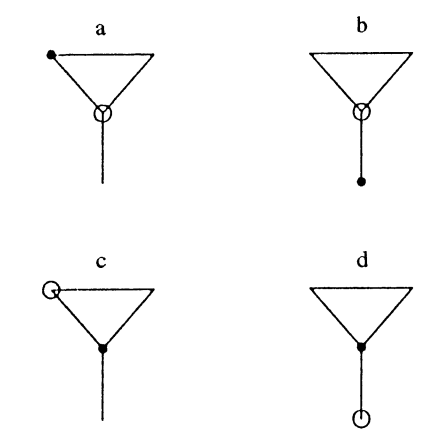
\includegraphics[scale = 0.5]{SpecialGraphCases}
\caption{Random walk on the special graph \protect\cite{BG}}
\label{fig:specialGraphCases}
\end{figure}

Combining the cases enumerated above, we obtain the following equation, where 1 represents the step already taken to reach one of the vertices

\begin{equation}
m_{13} = 1 + \frac{2}{3} \cdot a + \frac{1}{3} \cdot b
\end{equation}

If we allow the particle to continue its walk from its current vertex until three vertices have been visited, we can calculate remaining times that correspond to the graphs in figure \ref{fig:specialGraphCases}. Thus, we have the four following additional equations

\begin{equation}
\begin{alignedat}{2}
    a &= 1 + \frac{1}{2} \cdot 0 + \frac{1}{2} \cdot c \qquad
    &b &= 1 + d \\
    c &= 1 + \frac{2}{3} \cdot 0 + \frac{1}{3} \cdot a \qquad
    &d &= 1 + \frac{2}{3} \cdot a + \frac{1}{3} \cdot b
\end{alignedat}
\end{equation}

Each letter in these equations represents the particle being positioned according to the corresponding illustration, and a 0 means the particle has reached 3 vertices and requires no additional traversing across the graph. Each coefficient represents the likelihood that the particle will choose each vertices (accounting for symmetry). 

If we plug these four equations into the original partial cover time equation, we find that \textit{$m_{13} = 16/5$}. Using this general strategy, we can derive similar equations to compute the cover time, partial cover times, extended cover time, and extended partial cover times on this special graph. Used on larger, more complicated graphs, this strategy quickly becomes tedious. To demonstrate this, we briefly study the following example: let the particle rest on the eight corners of a cube - compute the mean number of steps required to pass across all eight edges. Although ostensibly simple, this computation involves a system of equations of 387 unknowns (compared to five unknowns in our special graph).

If we place a king somewhere on an empty chessboard, how many random moves does it take for him to reach all 64 squares? Clearly a system of equations would be futile, but we can make a strong estimate of the expected value by calculating the mean of a large number of trials. Using a simulation I created of a 250 thousand trials, the mean cover time of a king is 615 moves. If we put a knight through the same experiment, we get a mean of 556 moves. 

\begin{figure}[H]
\centering
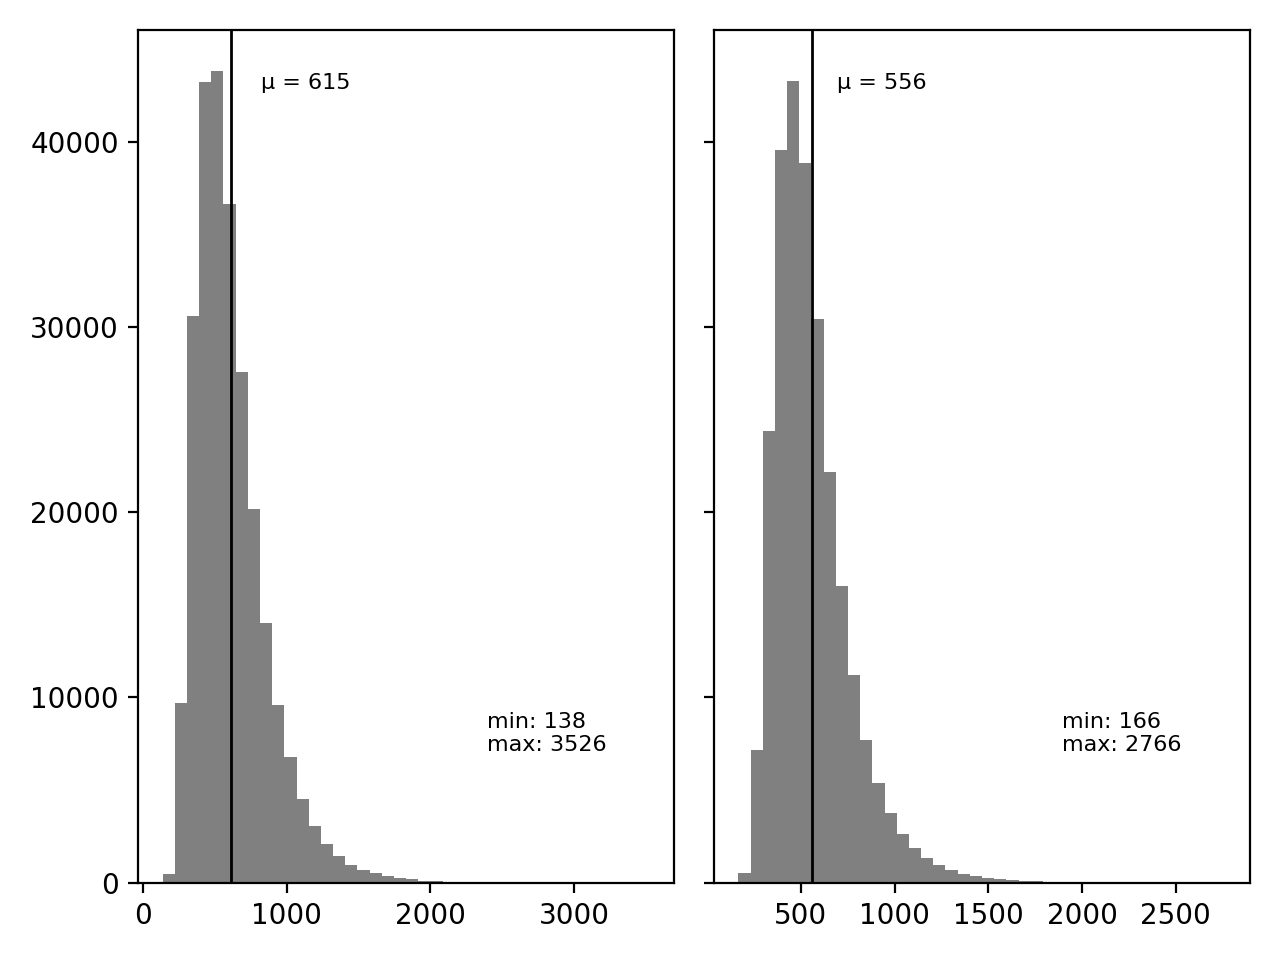
\includegraphics[scale = 0.5]{chessdistrs}
\caption{Random walk of a king and a knight on an empty chessboard, where the initial position is chosen at random.}
\end{figure}

The main method of this code can be found in the appendix. It may come as a surprise to readers that a knight has a smaller mean value. Although we won't use simulation to determine any more cover times in this paper, I thought that this chess board example might serve as a simple yet relatable example of a cover time, and that the result of my simulation might be found interesting. 
 \cite{BG}






\subsection{Polygons}

\indent \indent Next, we consider a polygon with \textit{n} vertices, numbered 0, 1, ... , \textit{n}-1. A particle starts at vertex 0 and moves to one of the two adjacent corners, 1 or \textit{n}-1 in this case. This binary choice occurs at time \textit{t} = 2, 3,... until all \textit{n} vertices have been visited. 

In order to compute cover time and extended cover time, we can consider the polygonal graph equivalent to a walk on the x-axis, starting at zero. A hexagon, for example, is equivalent to a number line with range [-5,5]. The starting vertex is now the origin, and each corner 1, ... , n - 1 is now represented twice - corner 1 is now 1 and -5 on the number line, corner 2 is now 2 and -4, and so on. The walk on the number line continues until the \textit{range} of the walk becomes 6. This is equivalent to a particle reaching all corners on a polygon of \textit{n} = 6. The general case for this transformation will be used to prove the expected time until absorption. 

Consider a classical symmetric walk that starts at the point 0, with absorbing barriers $a$ and $b$. The average time until one of these points is reached is equal to $ab$. Although this result is not proved here, we will use it to prove the expectation of $T_{i}$ - the amount of time it takes for the number of points visited to increase to a given number $i$. Consider a particle's path up to $t = 8$ is

\begin{equation}
0 \to 1 \to 0 \to 1 \to 2 \to 1 \to 0 \to -1.
\end{equation}

\noindent Here, $T_{1}$ = 0, $T_{2}$ = 1, $T_{3}$ = 5, and $T_{4}$ = 8. The range of this walk at \textit{t} = 8 is 4. \newline
\\
\indent Suppose that, at time $T_{i}$, the range is [-i+k+1, k], and the particle is positioned at the rightmost point \textit{k}. At time $T_{i+1}$, the particle is just outside this range, at either \textit{-i+k} or \textit{k}+1. The distance to these points are i and 1, respectively, making the expected time to reach either of these points $1 \cdot i$, by the classical symmetric walk quoted earlier. Thus we have proved 

\begin{equation}
E(T_{i+1}) - E(T_{i}) = i
\end{equation}

\noindent By this recursive definition, we get

\begin{equation}
E(T_{i}) = 1 + 2 + ... + (i-1) = \frac{1}{2}i(i-1)
\end{equation}

\noindent Remembering our goal to find the cover time of a polygonal graph, we get the result 

\begin{equation}
m_{n} = E(T_{n}) = \frac{n(n-1)}{2}
\label{eq:polygonCover}
\end{equation}

This result holds for all starting positions of the particle. Only the number of vertices $n$ is relevant.
\\

Finding the extended cover time $u_{n}$ is more complicated. We want to find an expression for the absorption time, and add this to the cover time we just determined. Thus we get the sum

\begin{equation}
u_{n} = m_{n} + c_{n},
\label{eq:polygonExCover}
\end{equation}

\noindent where

\begin{equation}
c_{n} = \sum_{j=1}^{n-1} c_{nj} p_{j}
\end{equation}

Here, $p_{j}$ is the probability that, at $m_{n}$, the particle is at point \textit{j}, and $c_{nj}$ is the expected absorption time. For all vertices \textit{j}, regardless of their distance from the starting vertex, $p_{j} = 1/(n-1)$. It may come as a surprise that the particle is not less likely to end up at a vertex close to the starting point than one further away, but it is indeed true. 

We consider different alternatives for the range at time $T_{i}$. We can denote $R_{i}$ the range of the particle at time $T_{i}$. There are always \textit{i} alternative ranges for $R_{i}$, which are as follows. Clearly, at time $T_{i}$, the particle is at either end point of the range.

 \begin{equation}
A_{0} = [-i + 1, 0]; A_{1} = [-i + 2, 1]; . . . ; A_{i-1} = [0, i - 1]
\end{equation}

We now wish to prove that these alternatives occur with equal probability $1/i$. To prove this, we consider the resting point of the particle at $T_{i}$. For each alternative, the particle could be resting at either end point. We can denote these possibilities as pairs of events $(A_{0}^{+}, A_{0}^{-}), ... , (A_{i-1}^{+}, A_{i-1}^{-})$, where $A_{0}^{+}$ indicates that the particle is at the right end point of the range $A_{0}$ at $T_{i}$, and $A_{0}^{-}$ indicates that it is on the left end point. 

Consider the general case of these pairings, a pair $(A_{k}^{+}, A_{k}^{-})$, where the range is defined as

 \begin{equation}
A_{k} = [-i + k + 1, k]
\end{equation}

\noindent Clearly, in order for event $A_{k}^{+}$ to occur, the particle must visit point $-i + k + 1$ before point $k$. This occurs, thanks to a proof not included in this paper, with probability 

\begin{equation}
\frac{k}{k + (i - k - 1)} = \frac{k}{i - 1}
\end{equation}

\noindent Additionally, the particle must visit point $k$ before point $-i + k$ in order for event $A_{k}^{+}$ to occur. This occurs with probability 

\begin{equation}
\frac{1}{k + (i - k)} = \frac{1}{i}
\end{equation}

\noindent Thus, by multiplying these probabilities together, we get

\begin{equation}
P(A_{k}^{+}) = \frac{k}{i - 1} \cdot \frac{1}{i}.
\end{equation}

\noindent By a similar proof on the left side of the range, we get

\begin{equation}
P(A_{k}^{-}) = \frac{i - k - 1}{i - 1} \cdot \frac{1}{i}.
\end{equation}

\noindent If we add these two equations together, we get the overall probability of $A_{k}$, namely

\begin{equation}
P(A_{k}) = \frac{1}{i},
\end{equation}

Since there are $n - 1$ possible values for $i$ in a polygonal graph with $n$ edges, we have proven that $p_{j} = 1/(n-1)$. 
\\
\\
\indent Now we wish to determine the expected amount of time for a particle to return from point $j$ to the starting vertex, which we denoted $c_{nj}$ earlier. This is again equivalent to a random walk on the x-axis from point $j$ and stopping at a point $j$ steps to the right or $n - j$ steps to the left. The expected time until absorption in this case is $c_{nj} = j(n-j)$. Thus we have 

\begin{equation}
c_{n} = \sum_{j=1}^{n-1} j(n - j) \cdot \frac{1}{n - 1} = \frac{n(n + 1)}{6}
\label{eq:polygonAbs}
\end{equation}

\noindent If we add (\ref{eq:polygonCover}) and (\ref{eq:polygonAbs}) into (\ref{eq:polygonExCover}), we get 

\begin{equation}
u_{n} = \frac{n(n-1)}{2} + \frac{n(n + 1)}{6} = \frac{n(2n - 1)}{3},
\end{equation}

\noindent which is the correct extended cover time for an $n$-sided polygonal graph.
\cite{BG}






\subsection{Complete Graphs}

\indent \indent A type of graph that presents a simple cover time computation is the \textit{complete graph}, in which each vertex is connected to every other vertex in the graph by a single edge. That is, a particle on the graph can reach any vertex from any other vertex in just one move. We denote the cover time of a complete graph \textit{$m_{n}$}, as the starting vertex does not matter due to symmetry.

\begin{figure}[h]
\centering
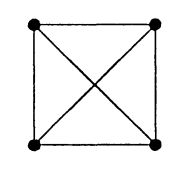
\includegraphics[scale = 0.8]{CompleteFour}
\caption{A complete graph with four vertices.}
\label{fig:CompleteFour}
\end{figure}

To derive the cover time of a complete graph of size \textit{n}, we use a simple trick. We can write

\begin{equation}
m_{n} = E[Y_{1}] + E[Y_{2}] + ... + E[Y_{n}],
\end{equation}

where $E[Y_{j}]$ is the expected amount of time required for the number of visited vertices to go from \textit{j} - 1 to \textit{j}. The amount of moves required to reach one more vertex has the geometric probability function 

\begin{equation}
P(Y_{j} = k) = (1-p_{j})^{k-1}p_{j}, \quad k = 1, 2, \ldots
\end{equation}

For $k = 1, 2, \ldots$, with $(1-p_{j})^{k-1}$ representing the probability that the particle will remain in the set of visited vertices for \textit{k} - 1 moves, and $p_{j}$ the probability of the particle traveling to a new vertex on move \textit{k}.  At time \textit{k} - 1, the particle has visited $(j - 1)$ vertices, out of \textit{n}, thus $p_{j} =  [n - (j - 1)]/n$. Using the mean of a geometric distribution, we get

\begin{equation}
E[Y_{j}] = \frac{1}{p_{j}} = \frac{n}{n-j+1},
\end{equation}

\noindent and so

\begin{equation}
m_{n} = (n-1)\bigg(1 + \frac{1}{2} + ... + \frac{1}{n-1}\bigg).
\end{equation}

Using this equation, we can solve for the cover time of the complete graph in figure \ref{fig:CompleteFour}, and we get $m_{4} = 33/6$. 
\cite{BG}



\subsection{Cover Time Distribution of a Complete Graph}

\begin{figure}[h]
\centering
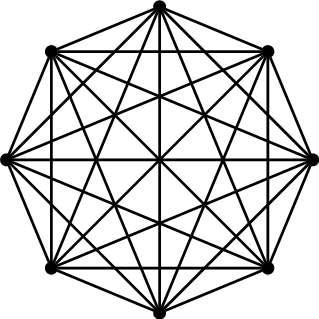
\includegraphics[scale = 0.3]{CompleteGraph}
\caption{A Complete Graph with 8 vertices}
\label{fig:CompleteEight}
\end{figure}

\indent \indent What if we are interested in the \textit{distribution} of this cover time variable, which we define as $\tau_{cov}$. Consider a complete graph of size $n$ with \textit{self-edges} - a particle on a given step can stay at it's current vertex. An example of such a graph is a man randomly dropping $r$ balls into $n$ boxes - each box is a vertex and each ball is an edge connected the previous box to the next one. Clearly, each of the $n^{r}$ possible arrangements occurs with equal probability. If we consider $N_{n}$ the number of empty boxes, and $A_{i}$ the event that box $i$ is empty, we clearly have

\begin{equation}
P(A_{i}) = (1 - 1/n)^{r} \quad \text{and} \quad E[N_{n}] = n(1 - 1/n)^{r}.
\end{equation}

\noindent We can show that if $rn \to c$, $E[N_{n}] \to e^{-c}$ using logarithms as follows

\begin{equation}
 E[N_{n}]/n = (1 - 1/n)^{r} = [(1 - 1/n)^{n}]^{r/n} \to (e^{-1})^{c} = e^{-c}
\end{equation}

In order to compute the variance of $N_{n}$, we need to find both $E[N_{n}]^{2}$ and $E[N_{n}^{2}]$. We define $\mathds{1}_{i}$ to be the indicator random variable of $A_{i}$, so $\mathds{1}_{i} = 1$ if box $i$ is empty and 0 otherwise. Starting with $E[N_{n}]^{2}$, we have

\begin{equation}
 E[N_{n}]^{2} = E\bigg[\bigg(\sum_{i=1}^{n}\mathds{1}_{i}\bigg)\bigg(\sum_{j=1}^{n}\mathds{1}_{j}\bigg)\bigg] = \sum_{1 \le i,j \le n}E[\mathds{1}_{i}]E[\mathds{1}_{j}] = \sum_{1 \le i,j \le n} P(A_{i})P(A_{j})
\end{equation}

\noindent Next we find $E[N_{n}^{2}]$

\begin{equation}
E[N_{n}^{2}] = E\bigg[\bigg(\sum_{i=1}^{n}\mathds{1}_{i}\bigg)^{2}\bigg] =  E\bigg[\bigg(\sum_{i=1}^{n}\mathds{1}_{i}\bigg)\bigg(\sum_{j=1}^{n}\mathds{1}_{j}\bigg)\bigg] = \sum_{1 \le i,j \le n}E[\mathds{1}_{i} \mathds{1}_{j}]= \sum_{1 \le i,j \le n}P(A_{i} \cap A_{j}).
\end{equation}


\noindent Using these to compute the variance of $N_{n}$, we get

\begin{align*}
var(N_{n})  &= E[N_{n}^{2}] - E[N_{n}]^{2} = \sum_{1 \le i,j \le n}P(A_{i} \cap A_{j}) - P(A_{i})P(A_{j}) \\
&= n(n - 1)\{P(A_{i} \cap A_{j}) - P(A_{i})P(A_{j})\} + n\{P(A_{i} \cap A_{j}) - P(A_{i})P(A_{j})\} \\
&= n(n - 1)\{(1 - 2/n)^{r} - (1 - 1/n)^{2r}\} + n\{(1 - 2/n)^{r} - (1 - 1/n)^{2r}\}.
\end{align*}

\noindent In the first term, $k \ne m$, and in the second term, $k = m$. We know, by logarithms, that $(1 - 2/n)^{r} \to e^{-2c} \quad \text{and} \quad (1 - 1/n)^{r} \to e^{-c}$. We can use this to determine, as $n \to \infty$,

\begin{align*}
\text{Var}(N_{n}/n)  &= \text{Var}(N_{n})/n^{2} \\
&= (1 - 2/n)^{r} (1 - 1/n)^{2r}  + o(n) \\
&\to e^{-2c} - (e^{-c})^{2} = 0.
\end{align*}

The second equality holds because, as $n \to \infty$, the second part of Var[$N_{n}$] becomes obsolete (we have denoted it $o(n)$). To conclude that $N_{n}/n \to e^{-c}$, we use Chebyshev's Inequality 

\begin{equation}
P(\vert N_{n}/n - E[N_{n}/n]\vert \ge \epsilon) \le \text{Var}(N_{n}/n)/\epsilon^{2}.
\end{equation}

\noindent We use this 
result to get

\begin{equation}
{N_{n}/n - E[N_{n}/n]} \xrightarrow{p} 0
\end{equation}

\noindent Here, $\xrightarrow{p}$ denotes convergence \textit{in probability}. We say that $Y_{n}$ converges to $Y$ in probability if $\forall \epsilon > 0, \text{ }P(\vert Y_{n} - Y \vert > \epsilon) \to 0  \text{ as } n \to \infty$. 
\medbreak

\noindent Plugging in our solved value of $E[N_{n}]$, we get

\begin{equation}
N_{n}/n - (1 - 1/n)^{r} \to 0 \quad \text{so} \quad N_{n}/n \to e^{-c}
\end{equation}

Thus, the fraction of empty boxes approaches $e^{-c}$. Based on the Poisson approximation to the binomial, we know that if $n \to \infty$ and $r/n \to c$,  that the number of balls in any given box approaches a Poisson distribution with mean $c$. Considering these results, we will now show, generalizing again to edges and vertices, 

\begin{thm}
If $ne^{r/n} \to \lambda \in [0, \infty)$, the number of unvisited vertices approaches a Poisson distribution with mean $\lambda$.
\label{thm:poisson}
\end{thm}

\begin{proof}
We start with the observation that $k$ unvisited vertices occurs with probability

\begin{equation}
P(\text{vertices } i_{1}, i_{2}, \ldots , i_{k} \text{ are unvisited}) = (1 - k/n)^{r}.
\label{eq:unvisitedVertices}
\end{equation}

Now we denote the probability that exactly $m$ out of $n$ vertices are empty after taken $r$ steps $p_{m}(r, n)$. Clearly $P($no unvisited vertices$) = 1 - P($at least one unvisited vertex$)$, so by inclusion-exclusion 

\begin{align}
p_{0}(r, n) &= {n \choose 0}1^{r} - {n \choose 1}(1 - 1/n)^{r} +{n \choose 2}(1 - 2/n)^{r} - \ldots \\
&= \sum_{k=0}^{n} (-1)^{k}{n \choose k}(1 - k/n)^{r}.
\label{eq:inclusionex}
\end{align}

Using the possibilities for different locations of unvisited vertices, we get a more sophisticated version of (\ref{eq:unvisitedVertices})

\begin{equation}
p_{m}(r, n) = {n \choose m}\bigg(1 - \frac{m}{n}\bigg)^{r}p_{0}(r, n - m)
\label{eq:unvisitedVertices2}
\end{equation}

To prove that the limit of $p_{m}(r, n)$ is a Poisson distribution with mean $\lambda$, we first need to prove that if $ne^{-r/n} \to \lambda$, then 

\begin{equation}
{n \choose m}\bigg(1 - \frac{m}{n}\bigg)^{r} \to \frac{\lambda^{m}}{m!}
\label{eq:squeeze}
\end{equation}

We can prove this using the squeeze theorem. We start with the upper bound. Since $(1 - x) \le e^{-x}$ and $ne^{-r/n} \to \lambda$, we have the inequality

\begin{equation}
{n \choose m}\bigg(1 - \frac{m}{n}\bigg)^{r} \le \bigg(\frac{n^{m}}{m!}\bigg)e^{-mr/n} \to \lambda^{m}/m!
\end{equation}

Now for the lower bound, which proves to be more difficult. We notice ${n \choose m} \ge (n - m)^{m}/m!$, and we use this to get

\begin{align*}
{n \choose m}\bigg(1 - \frac{m}{n}\bigg)^{r} &\ge \bigg(1 - \frac{m}{n}\bigg)^{r}\frac{(n - m)^{m}}{m!}\bigg(\frac{n^{m}}{n^{m}}\bigg) \\
&\ge \bigg(1 - \frac{m}{n}\bigg)^{m+r}\bigg(\frac{n^{m}}{m!}\bigg)
\end{align*}

We can use a couple tricks to simplify this. We know that, for a fixed $m$, $(1 - m/n)^{m} \to 1$ as $n \to \infty$, and that $1/m!$ is a constant. To bound the rest, we use a Taylor Series, noting that if $0 \le t \le 1/2$ then

 \begin{align*}
\log(1 - t) &= -t - t^{2}/2 - t^{3}/3 - \ldots \\
&\ge -t - \frac{t^{2}}{2}\bigg(1 + 2^{-1} + 2^{-2} + \ldots\bigg) = -t - t^{2}
\end{align*}

\noindent using this, we have

\begin{align*}
\log{\bigg(n^{m}\bigg(1 - \frac{m}{n}\bigg)^{r}\bigg)} &= m\log{n} + r\log{\bigg(1 - \frac{m}{n}\bigg)} \\
&\ge m\log{n} - r\bigg(\frac{m}{n}\bigg) - r\bigg(\frac{m}{n}\bigg)^{2}
\end{align*}

\noindent In order to solve for $r$, we use our assumption $ne^{-r/n} \to \lambda$,

\begin{align*}
e^{\log{n} - r/n} &\to e^{\log{\lambda}} \\
\log{n} - r/n &= \log{\lambda} + o(n) \\
r &= n\log{n} - \log{\lambda} + n\cdot o(n)
\end{align*}

\noindent from which we get $r(m/n)^{2} \to 0$. Now we can get

 \begin{align*}
\frac{rm}{n} &= m\log{n} - m\log{\lambda} + m \cdot o(n) \\
m\log{n} - \frac{rm}{n} &\to m\log{\lambda} 
\end{align*}

\noindent If we combine our last two results, we can show

\begin{equation}
\log{\bigg(n^{m}\bigg(1 - \frac{m}{n}\bigg)^{r}\bigg)} \ge m\log{n} - \frac{rm}{n} - \frac{rm}{n^{2}} \to \log{\lambda^{m}}
\end{equation}

\noindent From here, it follows that

\begin{equation}
\lim_{n \to \infty}n^{m}\bigg(1 - \frac{m}{n}\bigg)^{r} \ge \lambda^{m}
\end{equation}

Now we have proven (\ref{eq:squeeze}) via the squeeze theorem. Now we use (\ref{eq:inclusionex}) and (\ref{eq:squeeze}) to show that if $ne^{-r/n} \to \infty$, we have 

\begin{equation}
p_{0}(r,n) \to \sum_{k = 0}^{\infty} \frac{\lambda^{k}}{k!} = e^{-\lambda}
\end{equation}

Furthermore, we notice for a fixed $m$, $(n - m)e^{-r/(n-m)} \to \lambda$, so combining this with (\ref{eq:unvisitedVertices2}) and (\ref{eq:squeeze}), we get

\begin{equation}
p_{m}(r, n) = \frac{\lambda^{m}}{m!}e^{-\lambda}
\end{equation}

\noindent which is a Poisson distribution. So $N_{n}$ follows a Poisson distribution with mean $\lambda$, as claimed. 

\end{proof}

We can use Theorem \ref{thm:poisson} to learn about our cover time variable $m_{n}$ as well. If we set $r = n\log{n} + nx$, we get

\begin{equation}
ne^{-r/n} = ne^{-\log{n} - x} = \frac{ne^{-x}}{n} = e^{-x}
\end{equation}

Let's take, for example, a random walk of length $r$ on a complete graph with $n$ vertices. Clearly, $m_{n} \le r$ if and only if the particle covers all $n$ vertices in $r$ steps, and $ne^{-r/n} \to e^{-x}$, we have

\begin{equation}
P(m_{n} - n\log{n} \le nx) \to e^{-e^{-x}}.
\label{eq:birthdayhelp}
\end{equation}

\begin{exa}
What is the likelihood that, in a village of 2190 people, all possible birthdays are represented? What about a village of 1825?
\end{exa}
Consider this problem a cover time for a complete graph with 365 vertices, with each step representing a person in the group. With $n = 365$, we have $n\log{n} = 2153$. Plugging this into (\ref{eq:birthdayhelp}), we get

\begin{align*}
P(m_{365} \le 2190) &= P\bigg(\frac{m_{365} - 2153}{365} \le \frac{37}{365}\bigg) \\
&\approx e^{-e^{-0.1014}} = e^{-0.9036} = 0.4051 \\
P(m_{365} \le 1825) &= P\bigg(\frac{m_{365} - 2153}{365} \le \frac{-328}{365}\bigg) \\
&\approx e^{-e^{-0.8986}} = e^{-2.4562} = 0.085 
\end{align*}

So all birthdays being represented in villages of size 2190 and 1825 occurs with a 40\% and 8\% chance, respectively.
\\ \\
The analysis and results in this section follow from  \cite{DK}.




\section{Pólya's Reccurence Theorem}

\indent \indent In the early 1900s, Hungarian mathematician George Pólya was taking a walk in the park when he noticed he was passing the same couple often, even though it seemed as though they were both taking random paths through the park. Inspired, Pólya investigated the same problem on infinite graphs, eventually presenting his famous theorem in 1921, stating that a random walk on a $d$-dimensional lattice is reccurent for $d = 1, 2$, and transient for $d > 2$. We have introduced 1-dimensional random walks in section 1, but we will explore this further in famous problems Cliff Hanger. We will then look at the 2-dimensional and 3-dimensional cases in the Drunk Man and the Drunk Bird, respectively. The proofs of these problems follow from \cite{50}.

\subsection{One-Dimensional Random Walk: The Cliff-Hanger}

\indent \indent Suppose a man stands on the edge of a cliff - one step forward sends him over the edge. He takes random steps either toward or away from the cliff. At each given time, his chance of taking a step backwards is $\frac{2}{3}$, and his chance of taking a step forward is $\frac{1}{3}$. Will the man escape the cliff? 

We can view this problem as a particle walking along the x-axis, starting at $x = 1$. The particle visiting the origin is equivalent to the man stepping off the ledge. Clearly, the particle can only reach $0$ on an odd-numbered step, so we only consider these cases when computing the probability. At $t = 1$, the particle has a  $\frac{1}{3}$ of being at $0$. At $t = 3$, there is one possible way of reaching $0$: one step to the right and two steps to the left. This path occurs with probability $\frac{2}{27}$. At At $t$ = 5, the particle has two possible paths of reaching -1, namely 

\begin{equation}
1 \to 2 \to 1 \to 2 \to 1 \to 0 \text{ and } 1 \to 2 \to 1 \to 2 \to 1 \to 0
\end{equation}

\noindent each with probability $\frac{4}{243}$. Together, the particle has probability $\frac{107}{243}$ of reaching the origin at some point at or before time $t = 5$. We can continue adding up these possibilities for $t \to \infty$, but this is tedious - here is a simpler solution.

Let us look at the general case - the probability of a step to the right is equal to $p$, not $\frac{2}{3}$. Starting at index $x = n$, the particle moves to either $x = n+1$ with probability $p$ or to $x = n-1$ with probability $(1-p)$. We call $x = -1$ an \textit{absorbing barrier} - if the particle arrives there, it takes no further steps. We are interested in finding $P_{1}$ - the probability that the particle is \textit{absorbed} at $x = 0$, given that it starts at $x = 1$. At $t = 1$, the particle was absorbed with probability $(1 - p)$, and is at $x = 2$ with probability $p$. So we have

\begin{equation}
P_{1} = (1 - p) + pP_{2}
\label{eq:p1}
\end{equation}

Now let's look at $P_{2}$. Paths to absorption from $x = 2$ can be divided into two parts: the path from $2 \to 1$, and the path from $1 \to 0$. The first part is just $P_{1}$, because this problem is identical to the $1 \to 0$ case, just translated one step to the right. The second part is also $P_{1}$, because this is \textit{exactly} the original problem. So we then have $P_{2} = P_{1}^{2}$, because these two parts are independent. So we can rewrite (\ref{eq:p1}) as

\begin{equation}
P_{1} = (1 - p) + pP_{1}^{2}
\end{equation}

\noindent Solving this quadratic for $P_{1}$, we get solutions

\begin{equation}
P_{1} = 1, \quad P_{1} = \frac{1 - p}{p}
\end{equation}

Now we must determine when each of these solutions is appropriate. Let's look at a couple values of $p$ and think about what we'd expect $P_{1}$ to be. When $p = 0$, $P_{1}$ is obviously $1$, and when $p = 1$, $P_{1} = 0$, because the particle is always moving to the right. When $p = 0$, $P_{1} = 1$, and both solutions agree. When $p < \frac{1}{2}$, the second solution doesn't work because $(1-p)/p > 1$, and we know $P_{1} \le 1$. So we use the first equation $P_{1} = 1$ for $0 \le p \le \frac{1}{2}$. We can connect these two functions at $p = \frac{1}{2}$ and get the following graph

\begin{figure}[H]
\centering
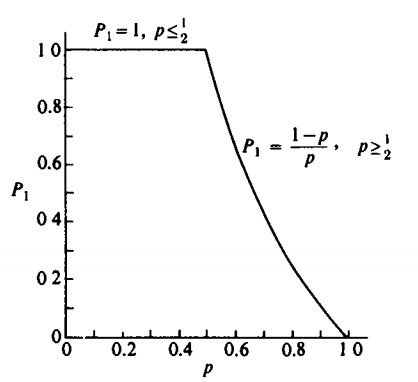
\includegraphics[scale = 0.8]{AbsorptionProbs}
\caption{Probabilities of absorption, $P_{1}$, of the Cliff-Hanger \protect\cite{50}}
\label{fig:AbsorptionProbs}
\end{figure}

A more thorough proof of this problem would include proving that the second solution, $P_{1} = (1 - p)/p$, is a continuous as a function of $p$. This is a result we will assume but not prove here. To answer our original inquiry, where $p = \frac{2}{3}$, we use the second solution, as $p > \frac{1}{2}$. We get $P_{1} = \frac{1}{2}$, which means the Cliff-Hanger's fall and escape from the cliff edge are equally likely.
\cite{50}





%\subsection{The Gambler's Ruin}
%
%Another interesting application of the 1-dimensional random walk is Gambler's Ruin. Here, two gamblers sit at a table. Player $M$ has \$1, and player $N$ has \$2. Every time a player wins, they get a dollar from the other player. Player $M$ is the stronger player, and wins 2/3 of the time. If the two gamblers play until one of them is bankrupt, what is the chance that player $M$ wins?
%
%To answer this question, let us generalize the problem. Players $M$ and $N$ have $m$ and $n$ units of currency, respectively. At each game, the probability of player $M$ winning is $p$, making $N$'s chances equal to $q = 1 - p$. As we did in Cliff Hanger, we visualize the problem as a particle on a number line. The particle starts at vertex $m$, and is absorbed at points 0 and $m + n$.
%
%If player $N$ has infinite resources, the problem becomes identical to the Cliff Hanger, and we inherit its result. We say the probability of absorption is equal to $(q/p)^{m}$. In the particle's path to absorption, it may visit vertex $m + n$. In the finite resources case, player $N$ becomes bankrupt here, ending the game. Let us denote the chances of the particle not reaching vertex $m + n$ before absorption $Q$. This is the chance of player $M$ losing. We have 
%
%\begin{equation}
%(q/p)^{m} = Q + (1 - Q)(q/p)^{m+n}.
%\label{eq:PandQ}
%\end{equation}
%
%Here, $Q$ represents the sequences that don't reach $m + n$, and $(1-Q)$ represents those that do, with $(q/p)^{m+n}$ being the proportion of these that make it back to zero if the game is allowed to continue indefinitely (if the game doesn't stop when player $N$ has lost). Since either $P$ or $Q$ must occur, we have $P + Q = 1$, and thus $P = 1 - Q$. If we substitute $P$ into (\ref{eq:PandQ}) and solve, we get
%
%\begin{equation}
%P = \frac{1 - (q/p)^{m}}{1 - (q/p)^{m + n}}.
%\label{eq:justP}
%\end{equation}
%
%If we use this to solve our original problem, with $p = 2/3$, $q = 1/3$, $m = 1$, $n = 2$, we get $P = 4/7$. Thus, player $M$ wins more often. 
%\\
%
%But if we set $p = q = 1/2$, wouldn't player $N$ be better off? If we plug these values into (\ref{eq:justP}), then $P$ becomes indeterminate, but if we apply L'Hospital's rule, we get
%
%\begin{equation}
%P = \frac{m}{m + n}, \quad \text{when}  \quad p = q = 1/2.
%\label{eq:justP}
%\end{equation}
%
%Thus $P = 1/3$, and $Q = 2/3$, making player $M$'s expectation 
%
%\begin{equation}
%E[M] = \frac{1}{3}(2) + \frac{2}{3}(-1) = 0
%\end{equation}
%
%Thus both players have expectation 0, making the game fair.
%\cite{50}



\subsection{Stirling's Approximation Proof}

\indent \indent As we progress into the 2-dimensional and 3-dimensional components of Pólya's Theorem, we see Stirling's Approximation used to deal with very large values of $n$. A very important formula in probability as well as in applied mathematics, it is used to approximate $n!$ as $n \to \infty$ . As I reference it in every section after this one, I saw fit to include its proof here. The work done in this proof closely follows from \cite{khamsi}.
\\

\noindent We start by taking the log of $n!$

\begin{equation}
\log{(n!)} = \log{(1)} + \log{(2)} + ... + \log{(n)}
\end{equation}

\noindent As the log function monotonically increases on the interval $(0, \infty)$, we know

\begin{equation}
\int_{n-1}^{n}\log{(x)}dx < \log{(n)} < \int_{n}^{n+1}\log{(x)}dx \quad \text{for all}\quad n > 1
\end{equation}

\noindent If we take the above inequalities for $n = 1, 2, ... , N$, and add them all together, we get

\begin{equation}
\int_{0}^{N}\log{(x)}dx < \log{(N!)} < \int_{1}^{N+1}\log{(x)}dx
\end{equation}

This first integral is improper, but convergent. Since the antiderivative of $\log{(x)}$ is equal to $x \log{(x)} - x$, we get

\begin{equation}
n\log{(n)} - n < \log{(n!)} < (n + 1) \log{(n+1)} - n
\end{equation}

\noindent Now we create a sequence $d_{n}$ such that

\begin{equation}
d_{n} = \log{(n!)} - \bigg(n + \frac{1}{2}\bigg)\log{(n)} + n
\end{equation}

\noindent Subtracting the $n+1$ term from the $n$th term, we get 

\begin{equation}
d_{n} - d_{n+1} = \bigg(n + \frac{1}{2}\bigg)\log{\bigg(\frac{n+1}{n}\bigg)} - 1
\end{equation}

\noindent Manipulating the algebra gives 

\begin{equation}
\frac{n + 1}{n} = \frac{1 + \frac{1}{2n + 1}}{1 - \frac{1}{2n + 1}}
\end{equation}

\noindent Now we implement the Taylor expansion to get 

\begin{equation}
\frac{1}{2}\log{\bigg(\frac{1+t}{1-t}\bigg)} = t + \frac{1}{3}t^{3} + \frac{1}{5}t^{5} + ... 
\end{equation}

\noindent so for $-1 < t < 1$, we get 

\begin{equation}
d_{n} - d_{n+1} = \frac{1}{3}\frac{1}{(2n + 1)^{2}} + \frac{1}{5}\frac{1}{(2n + 1)^{4}} + ... 
\end{equation}

\noindent which means 

\begin{equation}
0 < d_{n} - d_{n+1} < \frac{1}{3}\bigg(\frac{1}{(2n + 1)^{2}} + \frac{1}{(2n + 1)^{4}} + ... \bigg)
\end{equation}

\noindent which is a geometric series, so we can solve it to get 

\begin{equation}
0 < d_{n} - d_{n+1} <  \frac{1}{3}\frac{1}{(2n + 1)^{2} - 1}  = \frac{1}{12}\bigg(\frac{1}{n} - \frac{1}{n+1}\bigg)
\end{equation}

\noindent From this we have determined two things:
\begin{enumerate}
\item the sequence $d_{n}$ is decreasing
\item the sequence $d_{n} - \frac{1}{12n}$ is increasing
\end{enumerate}

\noindent Since both series converge, we can infer 

\begin{equation}
\lim_{x \to \infty} d_{n} = \lim_{x \to \infty} d_{n} - \frac{1}{12n} = C \quad \text{for some constant $C$}
\end{equation}

We know $C > d_{1} - 1/12 = 1 - 1/12 = 11/12$. Now we take the exponential of $d_{n}$, from which we get

\begin{equation}
\lim_{n \to \infty} \frac{n!}{n^{(n + 1/2)}e^{-n}} = e^{C}
\end{equation}

\noindent solving for $n!$, we get close to our desired approximation

\begin{equation}
n! \sim n^{(n + 1/2)}e^{-n} e^{C}
\label{eq:almostStirling}
\end{equation}


Now to prove $e^{C} = \sqrt{2\pi}$, we use the Wallis formula (the proof of which will thankfully not be included here), which states 

\begin{equation}
\lim_{n \to \infty} \frac{(2)(2)(4)(4)(6)(6)\cdot ... \cdot(2n)(2n)}{(1)(1)(3)(3)(5)(5)\cdot ... \cdot(2n-1)(2n-1)(2n+1)} = \frac{\pi}{2}
\end{equation}

\noindent We can rewrite this to get

\begin{equation}
\frac{(2)(4)(6)\cdot ... \cdot(2n)}{(1)(3)(5)\cdot ... \cdot(2n-1)\sqrt{2n}} \sim \sqrt{\frac{\pi}{2}}
\end{equation}

\noindent This can be simplified to

\begin{equation}
\frac{(2^{n}n!)^{2}}{(2n)!}  \frac{1}{\sqrt{2n}} \sim \sqrt{\frac{\pi}{2}}
\end{equation}

\noindent Plugging in our approximation for $n!$ given in (\ref{eq:almostStirling}), we get

\begin{equation}
\frac{2^{2n}(n^{2n+1}e^{-2n}e^{2C})}{(2n)^{(2n+1/2)}e^{-2n}e^{C}} \frac{1}{\sqrt{2n}} \sim \sqrt{\frac{\pi}{2}}
\end{equation}

\noindent From here, we can use very simple algebra to get

\begin{equation}
e^{C} \sim \sqrt{2\pi}
\end{equation}

\noindent Finally, we can plug this value of $e^{C}$ into (\ref{eq:almostStirling}) to get

\begin{equation}
n! \sim (\sqrt{2\pi})n^{n+1/2}e^{-n}
\label{eq:stirling}
\end{equation}

\noindent which is Stirling's Approximation! We will be using this result in future sections.
\cite{khamsi}





\subsection{Two-Dimensional Random Walk: The Drunk Man}
\medskip
\indent \indent A drunk man stumbles out of his house late one night. With no sense of direction, he travels northeast, northwest, southeast, and southwest with equal probability at every intersection. If the night is infinitely long, will the man become hopelessly lost, or will he eventually find his way back home?
\\

We can again view this problem as a random walk on a graph. In the 1-dimensional version of the random walk presented in the Cliff Hanger, we proved that returning to origin is unity when steps to the left and to the right are equally likely, but this was a special case. If the probability moves (even slightly) from $\frac{1}{2}$, this result no longer holds. Considering the set of roads and intersections to be an infinite lattice, and the drunk man a particle starting at the origin, it would seem that wandering off in two dimensions would be likely. To investigate this, we will compute the average number of times the particle returns, and deduce its probability of absorption from this. As we have in previous problems, we will denote a particle's probability of return $P$, and the probability of no return $Q = 1 - P$. The probability of exactly $x$ returns is simply $P^{x}Q$, as the walk just restarts every time the particle returns. We could use a geometric series to solve for $\mu$, namely

\begin{equation}
\mu = \sum_{x=0}^{\infty} xP^{x}Q,
\end{equation}

which would give us our result, except we're still missing the values of $P$ and $Q$. So we are tasked with determining these values. 

We know that, in a geometric distribution, the mean number of trials until the first success is the reciprocal of the probability of success. In this example, the particle not returning to the origin is considered to be the 'success', as it terminates the series. So the mean number of trials until a non-return is 1/$Q$, and the mean number of successes is 1/$Q$ - 1. If we set $Q = 1$, the mean number of successes becomes 0, and as $Q \to 0$, mean successes approaches infinity. Furthermore, there exists a bijection between values of $\mu$ and values of $Q$ - for every mean there exists a $Q$ and vice versa. So we just need to compute one to get the other, and we have chosen to compute $\mu$.

We can consider the direction chosen at each vertex a product of two binary decisions. That is, an evenly-weighted coin is flipped to determine the north-south component of the walk, and flipped again to determine the east-west component. If we think about the particle in this way, we can consider the two dimensional walk the product of two independent one dimensional walks, which we have seen before. 

Clearly, a return to the origin can only occur on an even-numbered step, so we focus on walks of even length. After two steps, the horizontal component of the walk has the distribution

\begin{equation}
P(X_{2} = -2) = \frac{1}{4} , \quad P(X_{2} = 0) = \frac{2}{4} , \quad P(X_{2} = 2) = \frac{1}{4}. 
\end{equation}

The vertical component of the walk has an identical distribution, and their joint PDF is

\begin{figure}[h]
\centering
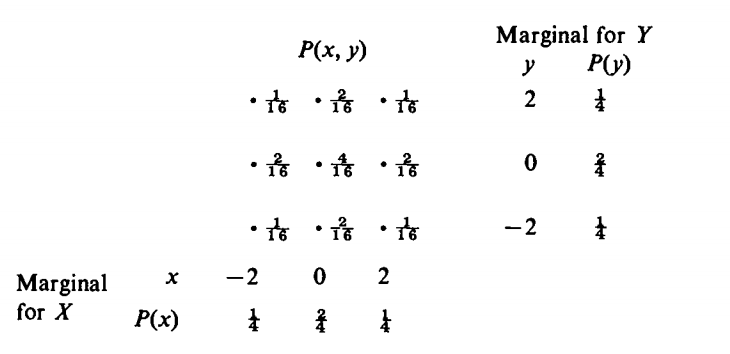
\includegraphics[scale = 1]{jointPDF}
\caption{Joint distribution of $X$ and $Y$ after two moves \protect\cite{50}}
\label{fig:jointPDF}
\end{figure}

We determine the probability that the particle rests at the origin after two moves to be $\frac{4}{16}$ by multiplying P(X = 0) together with P(Y = 0), which is possible because the two events are independent of one another. So far, our contribution to the mean is $1 \cdot (\frac{4}{16}) + 0 \cdot (\frac{12}{16}) = (\frac{4}{16})$. We can continue this computation for $n = 2, 4, 6, ... $ to get our final value for $\mu$, but it gets trickier from here on out. 
\\

Firstly, for all 1-dimensional even-length walks greater than 2, we have multiple ways of returning to the origin. For a walk of length 4, for example, we have 

\begin{equation}
0 \to 1 \to 0 \to 1 \to 0 \quad \text{ and } \quad 0 \to 1 \to 2 \to 1 \to 0 
\end{equation}

which both lead back to the vertex. We can count the number of returning walks of length $2n$ using binomial probabilities, and we get the overall equation

\begin{equation}
P(\text{return at step } 2n) =  P(X_{2n} = 0) \cdot P(Y_{2n} = 0) = \bigg[{2n \choose n}\bigg(\frac{1}{2}\bigg)^{2n}\bigg]^{2}.
\end{equation}

In order to determine this value, we apply Stirling's approximation (\ref{eq:stirling})

\begin{equation}
{2n \choose n}\bigg(\frac{1}{2}\bigg)^{2n} = \frac{(2n)!}{n! n!} \bigg(\frac{1}{2}\bigg)^{2n} \approx \frac{(\sqrt{2\pi})(2n)^{2n + \frac{1}{2}}e^{-2n}}{((\sqrt{2\pi})n^{n + \frac{1}{2}}e^{-n})^{2}2^{2n}} \approx \frac{1}{\sqrt{\pi n}}
\end{equation}

Squaring this result, we get

 \begin{equation}
P(X_{2n} = 0) \cdot P(Y_{2n} = 0) \approx \frac{1}{\pi n}
\end{equation}

Now that we have the approximate probability that a walk will return to the origin at step $2n$ for all values of $n$, we need to calculate the sum of all of these values. We get

\begin{equation}
\sum_{n=1}^{\infty} \frac{1}{\pi n} = \frac{1}{\pi} \sum_{n=1}^{\infty} \frac{1}{n}
\end{equation}

Since $\sum_{n=1}^{\infty} \frac{1}{n}$ diverges as $n$ grows, so does the probability that the particle returns at some even step. If we recall our goal, this is also the mean number of times the particle has returned to the origin after exactly $2n$ steps. Since this mean is unbounded, we know $P$, the probability that the particle will return, is equal to 1. Not only does the particle return, but it returns \textit{infinitely often}. Going back to our original problem, the drunk man will find his way home again. Upon arriving home, he could go for another walk, and infinitely more, and still end up home.
\cite{50}





\subsection{Three-Dimensional Random Walk: The Drunk Bird \vspace{1em}}

\textit{A drunk man will find his way home, but a drunk bird may get lost forever.}
\begin{flushright}
Shizuo Kakutani \quad \quad \quad
\end{flushright}

We have proven that a particle will return to the origin during both one-dimensional and two-dimensional random walks, so does it follow that it will return on a walk of $n$ dimensions? We start with the 3-dimensional case. An extension of our work in the previous section, we know that the chances of position of three  independent 1-dimensional walks equalling 0 is 

\begin{equation}
P(\text{return at step } 2n) =  P(X_{2n} = 0) \cdot P(Y_{2n} = 0) \cdot P(Z_{2n} = 0) = \bigg[{2n \choose n}\bigg(\frac{1}{2}\bigg)^{2n}\bigg]^{3}.
\end{equation}

\noindent Using Stirling's Aprroximation, we get

\begin{equation}
P(\text{return at step } 2n) \approx \frac{1}{(\pi n)^{\frac{3}{2}}}
\label{eq:sums}
\end{equation}

If we take the infinite series of these probabilities, we can use the identity $\sum_{n=1}^{\infty} \frac{1}{n^s}$ diverges for $s \leq 1$ and converges for $s > 1$. The three cases $d = 1, 2, 3$ considered in this paper correspond to $s = 1/2, 1, 3/2$. Thus the series diverge, diverge, and converge, respectively. Hence we have the result that a random walk of a particle is recurrent for $d = 1, 2$ (which we have proven in previous sections) and transient for $d = 3$ (a new result). Let us find the exact value of the absorption probability for $d = 3$. \\


Referring back to (\ref{eq:sums}), we can't use a series approximation for the sum of these values, but we can use an integral test to get a bound on the series. Visualize the sum $\sum_{n=0}^{\infty} 1/n^{3/2}$ as a series of rectangles of length 1 (from $n \to (n + 1)$) and height $1/(n^{3/2})$. Using the curve $f(x) = (n-1)^{\frac{-3}{2}}$, we have an upper bound that passes through the upper right-hand corners of each of the rectangles. Because this function is an upper bound, the area under the curve is greater than the sum of the areas of the rectangles. 


\begin{figure}[H]
\centering
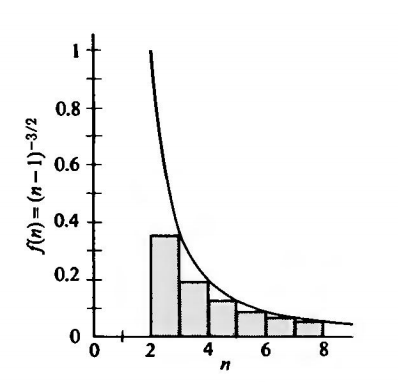
\includegraphics[scale = 1]{UpperBound}
\caption{Upper bound for $\sum_{n=0}^{\infty} \frac{1}{n^{3/2}}$ \protect\cite{50}}
\label{fig:UpperBound}
\end{figure}


\noindent Taking the integral, we get 

\begin{equation}
\int_{n}^{N} (n-1)^{\frac{-3}{2}} dx = -2(x - 1)^{\frac{-1}{2}} \bigg\rvert_{n}^{N} = \frac{2}{(n - 1)^{\frac{1}{2}}} - \frac{2}{(N - 1)^{\frac{1}{2}}}
\end{equation}

So as $N \to \infty$, this area approaches $2/(n - 1)^{\frac{1}{2}}$, which is finite, making the sum of the rectangles finite as well. We can evaluate the number by taking the sum of the series for a small number of $n$, and then approximating remainder of the integral using Stirling's Approximation. If we choose to sum the first 18 terms, we get

 \begin{equation}
\sum_{n=0}^{18} \bigg[{2n \choose n}\bigg(\frac{1}{2}\bigg)^{2n}\bigg]^{3} \approx 0.315,
 \end{equation}
 
\noindent and Stirling Approximation of the remainder of the integral is so small as to be considered negligible. Thus, 0.315 is approximately the mean number of returns to the origin of a given particle. Since $1/Q = 1 + \mu$, we solve for $Q$ and get $Q \approx 0.761$. We then can calculate $P$, the probability of a particle returning, to be approximately 0.239.

So a particle is more likely to wander off forever in three dimensions than return to the origin. It should come as no surprise to the reader that a walk in additional dimensions yields an even more improbable return. Using the same summation strategy, we find the probability of returning to the origin in a 4-dimensional walk to be approximately 0.105. These probabilities continue to decrease as the number of dimensions increases. 
\cite{50}

\newpage

\bibliography{Thesis2.1.bib}
\bibliographystyle{Thesis2.1.bib}
\nocite{*}

\newpage

\newgeometry{left=2cm}
\appendix
\label{appendix}
\section{Random Walk on a Chessboard: Source Code}
\nopagebreak
\small{
\begin{lstlisting}[language=Java]

public class Main {
    static int dims = 8; // dimensions of the chessboard (dims x dims)
    static int trials  = 1000000; // trials

    public static void main(String[] args){
        Random r = new Random();

        /*
        * Random walk of a king
        * */

        int[] kingTimes = new int[trials];
        for (int i = 0; i < kingTimes.length; i++) {
            Board b = new Board(dims);
            int randX = r.nextInt(dims);
            int randY = r.nextInt(dims);
            Square initSquare = b.getSquare(randX, randY);

            King myKing = new King(initSquare);
            initSquare.put(myKing);

            int numMoves = 0;
            while (!b.covered()) {

                LinkedList<Square> possibleMoves = myKing.getPossibleMoves(b);
                int ran = r.nextInt(possibleMoves.size());
                Square move = possibleMoves.get(ran);
                myKing.move(move);
                numMoves++;
            }
            kingTimes[i] = numMoves;
            System.out.println(numMoves);
        }

        /*
        * Random walk of a knight
        * */
        int[] knightTimes = new int[kingTimes.length];
        for (int i = 0; i < knightTimes.length; i++) {
            Board b = new Board(dims);
            Square[][] array = b.getSquareArray();
            int randX = r.nextInt(dims);
            int randY = r.nextInt(dims);
            Square initSquare = b.getSquare(randX, randY);

            Knight myKnight = new Knight(initSquare);
            initSquare.put(myKnight);

            int numMoves = 0;
            while (!b.covered()) {
                LinkedList<Square> possibleMoves = myKnight.getPossibleMoves(b);
                int ran = r.nextInt(possibleMoves.size());
                Square move = possibleMoves.get(ran);
                myKnight.move(move);
                numMoves++;
            }
            knightTimes[i] = numMoves;
            System.out.println(numMoves);
        }


        int kingSum = 0;
        int knightSum = 0;
        for (int i = 0; i < kingTimes.length; i++){
            kingSum += kingTimes[i];
            knightSum += knightTimes[i];
        }

        double kingAverage = kingSum/kingTimes.length;
        double knightAverage = knightSum/knightTimes.length;

        System.out.println("Mean cover time of a king on a chessboard (" + 
        		kingTimes.length + " trials): " + kingAverage + " moves");
        System.out.println("Mean cover time of a knight on a chessboard (" + 
        		knightTimes.length + " trials): " + knightAverage + " moves");

    }
}

\end{lstlisting}
}
\restoregeometry
\end{document}


